% ==================================
% ==================================
%  Kapitel 4 - Mathematische Formeln
% ==================================
% ==================================


\chapter{Implementation}
\label{ch:implementation}

In this chapter, we move from system design (Chapter~\ref{sec:system_design}) to the concrete realization of our pipeline.  We detail how each component was implemented in practice from data extraction from the HDF5 files using region masks and custom scripts to signal preprocessing for spectrogram generation culminating in model training with various data augmentation techniques and checkpointing. Discussion on how the specific libraries and frameworks adopted, the structure of key code modules, configuration parameters, and the strategies employed to validate and manage intermediate outputs, providing a clear, end-to-end account of how the system was built, tuned, and prepared for deployment.  


\section{Extraction of Footstep and Background Data}
Data collected from the setup explained in section~\ref{sec:experimental_setup} is stored in the HDF5 file. HDF5 file is visualized as explained in section~\ref{sec:data_acquisition} and shown in Figure~\ref{phase_plot}. Region masks are used to extract the footstep and background with the help of annotations on RGB plot of the HDF5 file. RGB plot is used to enhance the visual interoperability, for which a Short-Time Fourier Transform (STFT) in tandem with a custom-designed filter bank. The application of a logarithmic transformation further enhances the visualization, making subtle patterns more evident. Figure~\ref{labelme} provides an illustrative RGB image of the raw phase data where the horizontal axis corresponds to the distance along the cable route and the vertical axis represents time, with time progressing from the top (earliest) to the bottom (latest). The RGB plot is opened using the LabelMe tool. 

\begin{figure}[h]
    \centering
    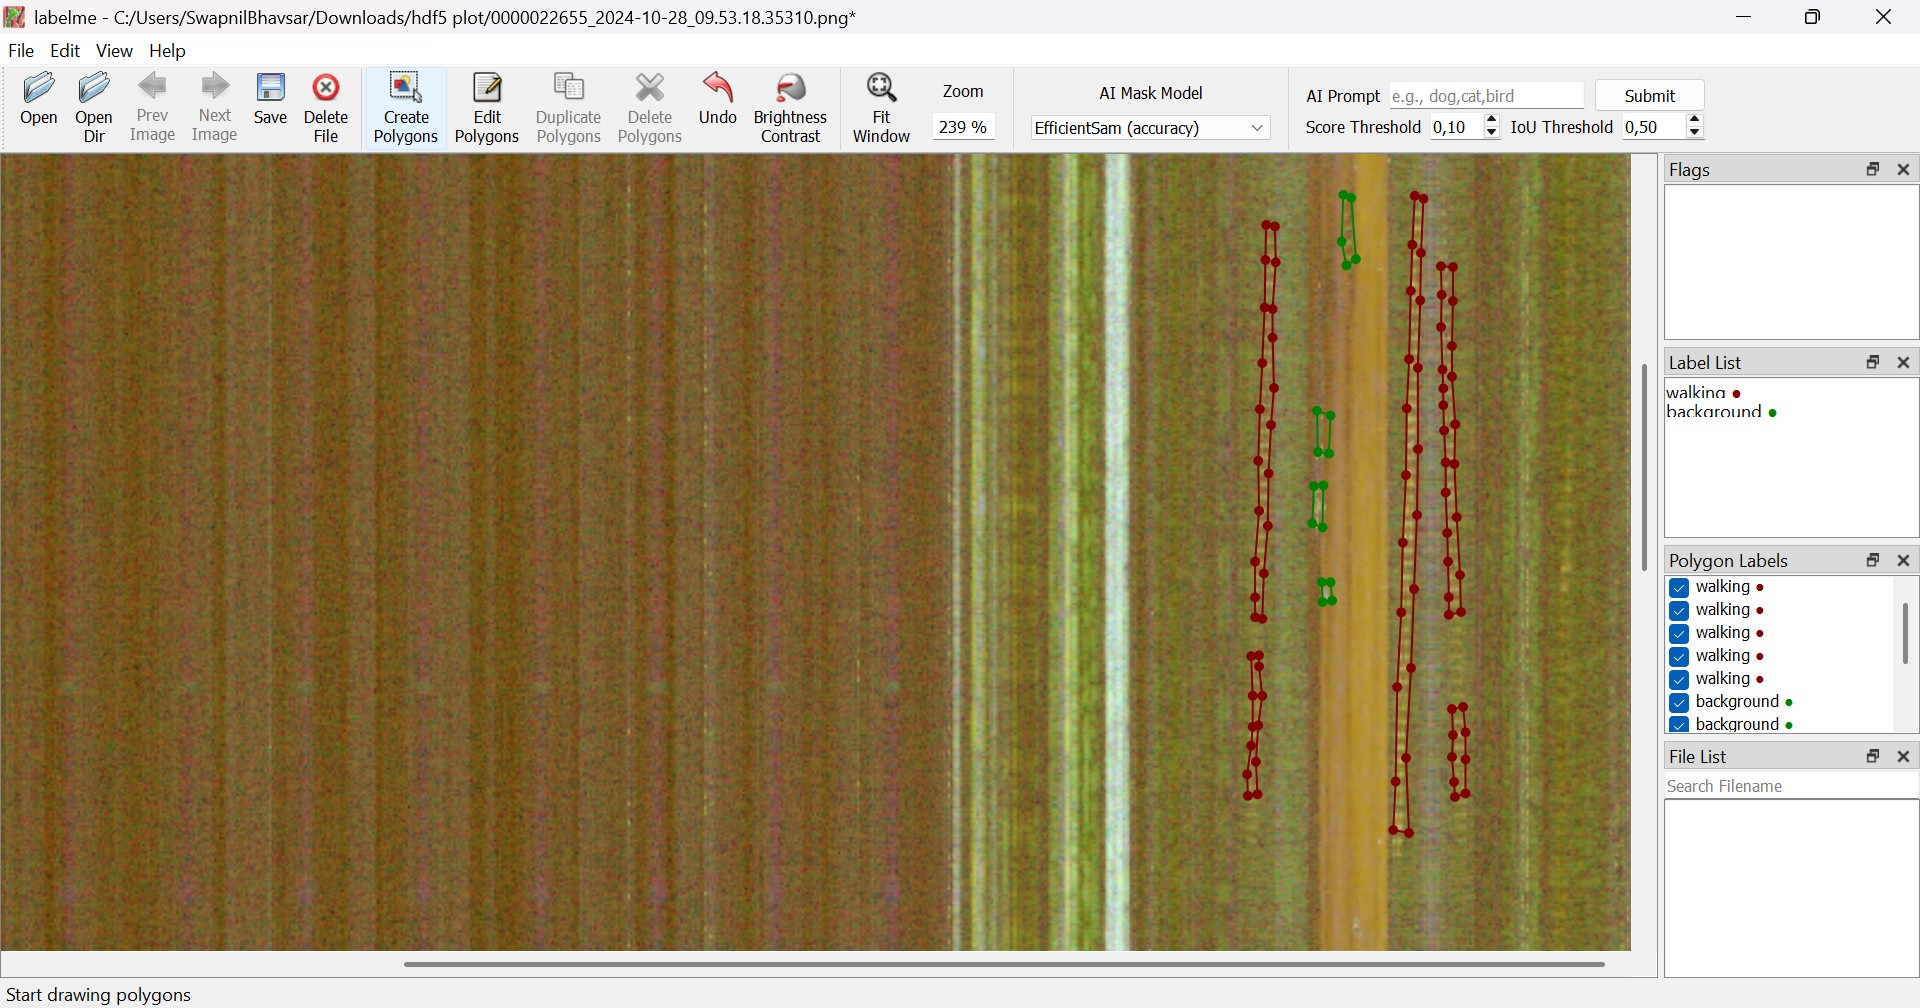
\includegraphics[width=\linewidth]{Bilder/jpg/label.jpg}
    \caption{LabelMe tool for annotation}
    \label{labelme}
\end{figure}

RGB plot has footsteps trails in it and we need to annotate it and extract the footsteps data using the RGB plot and HDF5 files. LabelMe tool is used to annotate the footsteps trail in RGB plot. LabelMe tool is a open-source image annotation tool that allows users to draw polygons on images and generate JSON files containing the binary masks corresponding to the annotated regions. The class labels are also added to the annotated regions. The extraction blocks takes the JSON masks and the HDF5 file which is used to extract the footstep data from the HDF5 file and store it in .npy or .bin file~\cite{Labelme}. Figure~\ref{labelme} shows the window for the LabelMe tool. It contains a RGB plot for HDF5 file. It contains option to draw the polygons for the exact part which is needed for the dataset. Figure~\ref{labelme} has two different colors of polygons where red polygon is used to annotate footstep data and the green polygon is used to annotate the background data.

The output from Labelme includes JSON files, which contain binary masks corresponding to the annotated regions. A custom script is then used to extract the appropriate raw phase data segments from the HDF5 files by applying the binary masks. Listing~\ref{lst:core_extraction} presents the core function that embodies the sample extraction process.

\begin{lstlisting}[style=pythonstyle, caption={Core logic for extracting samples from a mask}, label=lst:core_extraction]
def extract_samples_from_mask(mask, data_array, data_rate_hz, 
                    window_len_sec, window_width_channels):
    window_length_traces = int(data_rate_hz * window_len_sec)
    hop_size_time = int(window_length_traces * 0.5)
    hop_size_space = max(1, int(window_width_channels * 0.5))
    
    actual_mask = mask[::-1]
    col_has_label = np.any(mask, axis=0)
    row_has_label = np.any(mask, axis=1)
    left_start = np.argmax(col_has_label)
    right_end = len(col_has_label) - np.argmax(col_has_label[::-1])
    top_start = _DOWNSAMPLE_FACTOR * np.argmax(row_has_label)
    bottom_end = _DOWNSAMPLE_FACTOR * (len(row_has_label) - np.argmax(row_has_label[::-1]))
    
    for start_x in range(max(0, left_start - hop_size_space), 
                            right_end - hop_size_space, hop_size_space):
        for start_y in range(max(0, top_start - hop_size_time), 
                             bottom_end - hop_size_time, hop_size_time):
            chunk = data_array[start_y : start_y + window_length_traces, 
                                start_x : start_x + window_width_channels]
            mask_chunk = actual_mask[start_y // _DOWNSAMPLE_FACTOR : 
                                    (start_y + window_length_traces) // _DOWNSAMPLE_FACTOR,
                                    start_x : start_x + window_width_channels]
            if chunk.shape != (window_length_traces, window_width_channels) or \
                np.mean(mask_chunk.astype(float)) < _REQUIRED_MASK_PROPORTION:
                continue
    \end{lstlisting}

In this function, several key computational steps are performed:
    \begin{itemize}
        \item The window length is calculated based on the data rate and the desired duration.
        \item A binary mask, generated from Labelme annotations, is processed to identify the columns and rows that contain labels.
        \item Nested loops are implemented to extract segments of the raw phase data along both spatial and temporal dimensions.
        \item The extracted segments, referred to as \texttt{chunk} and \texttt{mask\_chunk}, are then verified based on their shape and the proportion of the label mask present before being stored for further processing.
    \end{itemize}

The extracted files (.npy/.bin files) are stored in different directories based on the type of data (footstep or background) and the corresponding labels. Based on the labels, the data is divided into training and test sets. 
These sets are preprocessed before being used for training and testing the model. 

\section{Preprocessing of extracted Data}
\label{preproc}
Following extraction, the extracted files needs to be preprocessed so that the clear distinction between the footsteps and background data can be made. The distinction is seen in the form of spikes which is visible in footstep data in comparison to background data as seen in Figure~\ref{walking_1d} and Figure~\ref{bg_1d} from section~\ref{sec:preprocessing}.  The preprocessing is used to convert the raw phase data into a more interpretable format, specifically a spectrogram. This transformation is crucial for the subsequent training of the model, as it allows for the identification of patterns and features that are indicative of footstep events. The preprocessing pipeline is designed to handle the raw phase data efficiently, ensuring that the resulting spectrograms are both informative and suitable for machine learning applications. We use Scipy's signal tools~\cite{scipy2020} for filtering and STFT, torchaudio's Mel-scale filter banks~\cite{torchaudio2024}.

The preprocessing routine, as demonstrated in Listing~\ref{lst:mag_processing}, involves reading the extracted data files, executing the STFT, and finally converting the resulting power spectrum into decibel (dB) values. The transformation to a logarithmic scale is critical, as it optimizes the dynamic range of the visualized data and makes both prominent and subtle patterns more discernible. We employ the \texttt{Visualizer} class which is the custom created class for these operations in the listing~\ref{lst:mag_processing}. In its constructor we build a Mel-filter bank matrix via \texttt{melscale\_fbanks(...,~mel\_scale="htk",...)}, which yields finer resolution at low frequencies where footstep energy is concentrated and coarser resolution at high frequencies, improving both compactness and interpretability of the spectrogram. The method \texttt{\_accum} prepares raw data by taking a cumulative sum and then applying a high-pass filter to remove low-frequency drift. Finally, \texttt{preprocess} computes the STFT, squares the magnitude, and applies a $10\log_{10}(\cdot)$ transform to produce the final spectrogram. The logarithimic function make the spectrograms both visually clearer and more suitable to downstream classification. 

\begin{lstlisting}[style=pythonstyle, caption={Core processing for converting raw phase data to magnitude output}, label=lst:mag_processing]
class Visualizer:
   def __init__(self, data_rate_hz: int = 1000):
        self._data_rate_hz = data_rate_hz
        self._f_bank = (
            melscale_fbanks(
                n_freqs= 128 // 2 + 1,
                f_min=0,
                f_max=500,
                n_mels=64,
                sample_rate=data_rate_hz,
                mel_scale="htk",
                norm=None,
            )
            .cpu()
            .numpy()
        )

    def _accum(self, x: np.ndarray) -> np.ndarray:
        x = np.cumsum(x, axis=0, dtype=np.int64).astype(np.float32)*INT_TO_RADIANS
        sos = signal.butter(2, 5, "hp", fs=1000, output="sos")
        return signal.sosfiltfilt(sos, x, axis=0)

    def preprocess(self, data: np.ndarray) -> np.ndarray:
        data_accum = np.cumsum(data, axis=0)
        f, t, stft = signal.stft(
            data_accum, fs=self._data_rate_hz,
            nperseg=128, noverlap=114,
            padded=False, scaling="psd", axis=0
        )
        stft = np.abs(stft) ** 2
        stft = np.matmul(stft.T, self._f_bank).T
        mag = 10 * np.log10(stft)
        return mag
\end{lstlisting}

To facilitate the training of the deep learning models such as ConvNext V2 and EfficientNet. Two different models are trained so that a comparison can be made for their performances and accuracies, two separate datasets are generated through variations in the sample length and the number of spatial channels considered:
\begin{itemize}
    \item The first dataset employs a sample length of 1.728 seconds and uses only 1 spatial channel. Sample length of 1.728 seconds as it contains 3 to 4 steps and the dataset with same configuration as there are already recorded files available. Based on the models trained on these, it is useful to detect shorter as well as longer footstep trails. The processing pipeline for this dataset is executed using the extraction procedure from Listing~\ref{lst:core_extraction} and is subsequently converted into spectrograms following the process described in Listing~\ref{lst:mag_processing}. Figure~\ref{walking_1ch} illustrates the resulting spectrogram for walking data acquired through a single spatial channel. In this Figure, the upper plot corresponds to the phase plot which reveals the unwrapped phase variations over time, whereas the lower plot represents the corresponding STFT spectrogram. Noticeably, the distinct spikes present in the spectrogram mark the precise moments when a foot makes contact with the ground.
    
    \begin{figure}[h]
        \centering
        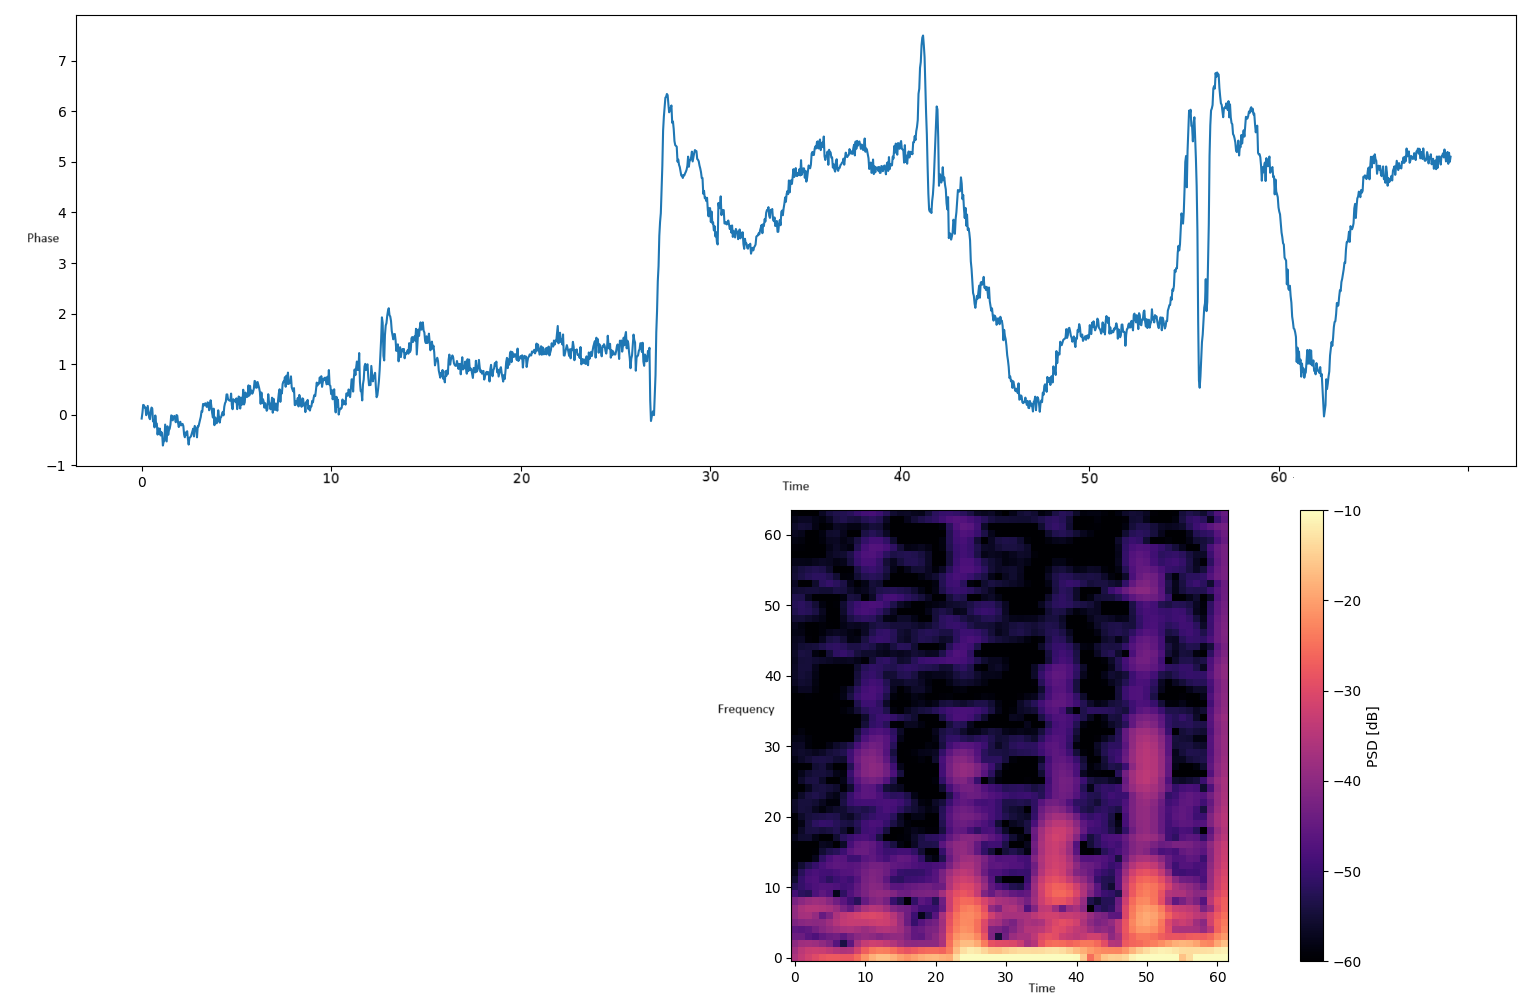
\includegraphics[width=0.8\linewidth]{Bilder/jpg/walking_1ch.png}
        \caption{Spectrogram for walking data with 1 spatial channel}
        \label{walking_1ch}
    \end{figure}

    \item The second dataset is designed for capturing more complex spatial and temporal interactions and uses a sample length of 2 seconds along with 10 spatial channels. The sample length of 2 seconds is taken which can be estimated as the time length in which a person can take 3 to 4 steps. The spatial channels record the data which are 5m apart. So the neighboring spatial channels record distortions based on the same footsteps and they can be detected many times by trained model. To avoid this 10 spatial channel are selected so model can exactly focus on footsteps and not the distortions in the neighboring spatial channels. The same extraction and preprocessing techniques are applied to this dataset. Figure~\ref{walking_10ch} shows that the top plot represents the distribution of the spatial channels over time, while the bottom plot highlights the frequency distribution. Importantly, files that lack clearly discernible footsteps are manually filtered out, ensuring that the final dataset is diverse and rich in footstep patterns. This deliberate filtering is paramount as it enhances the model's ability to generalize across various walking patterns and substantially reduces the occurrence of false detections.
\end{itemize}

\begin{figure}[h]
    \centering
    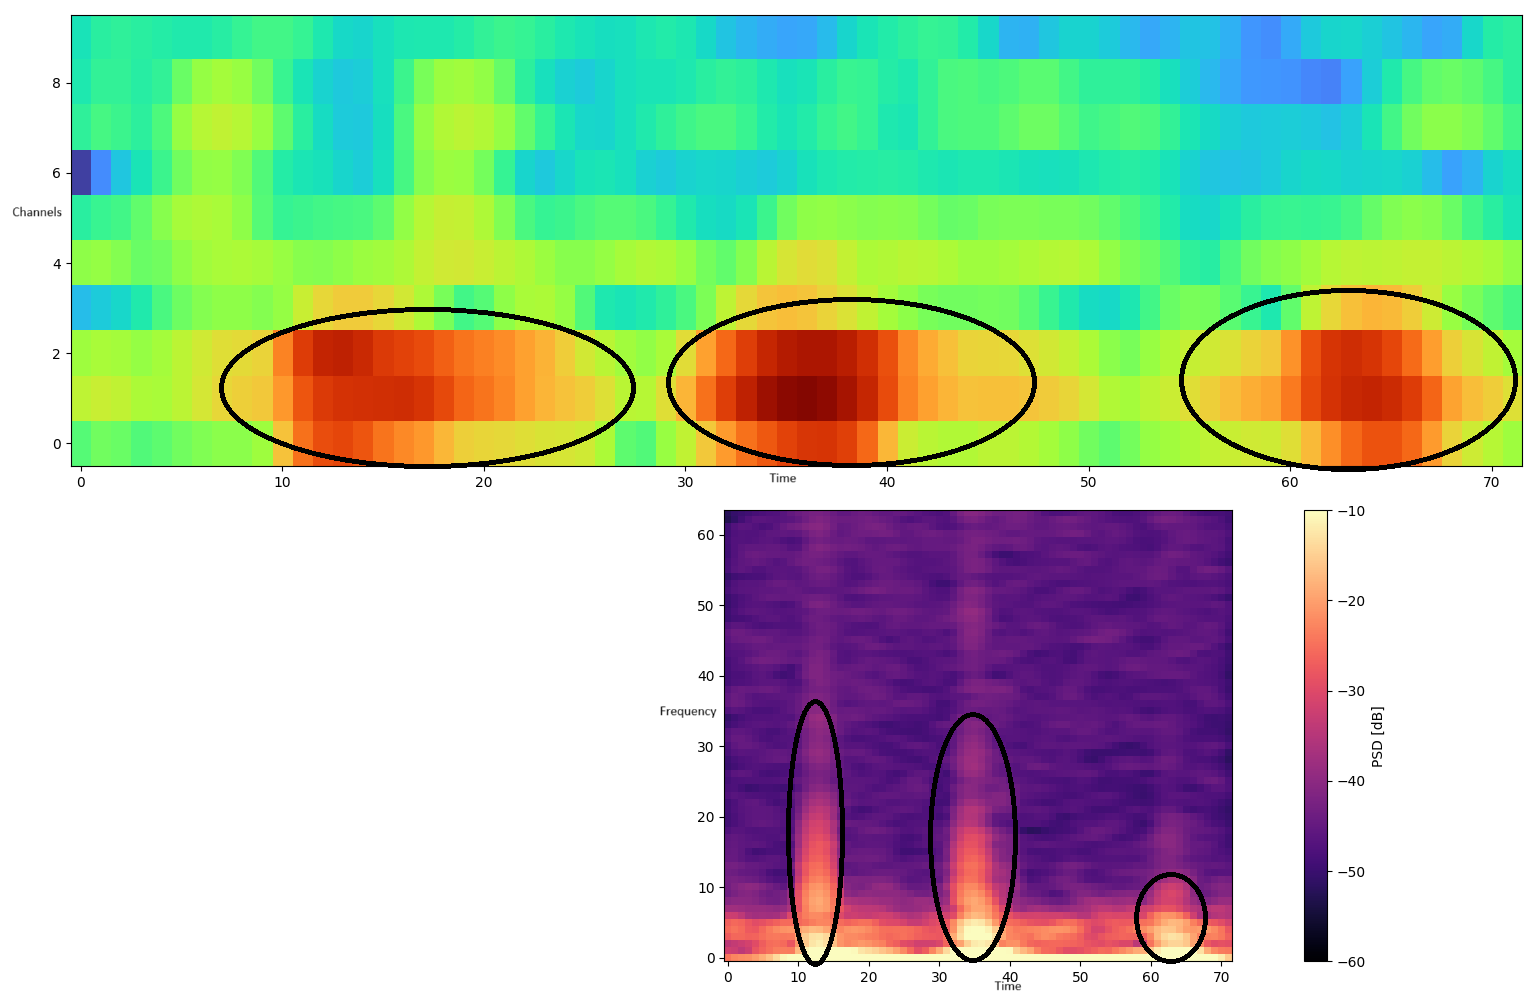
\includegraphics[width=0.8\linewidth]{Bilder/jpg/walking_10ch.png}
    \caption{Spectrogram for walking data with 10 spatial channels}
    \label{walking_10ch}
\end{figure}

\section{Dataset}
\label{sec:dataset}
The dataset is created with the help of preprocessing steps. The raw extracted files (.npy/.bin) are stored in the folder and before the dataset is loaded to train the model, the preprocessing steps are used. Dataset are of two types as described in the section~\ref{preproc}.

\begin {itemize}
\item \texttt{Dataset-1D}: 1.728 seconds sample length and 1 spatial channel
\item \texttt{Dataset-2D}: 2 seconds sample length and 10 spatial channels
\end {itemize}

Both datasets contains the \texttt{training} and \texttt{testing} folders which are used for the same purpose as the name suggests. Each of these folders has two folders \texttt{walking} and \texttt{background} which are different events that are used as labels for training the models.

\texttt{Dataset-1D} training folder 5818 walking samples and 2696 background samples. Testing folder for the same dataset contains 988 walking samples and 1590 background samples. \texttt{Dataset-2D} contains the same folders as \texttt{Dataset-2D} where training folder contains 1982 walking samples and 421 background samples. Testing folder contains 65 walking samples and 1682 bakcground samples.

\texttt{Dataset-2D} has much lesser samples compared to \texttt{Dataset-1D} because over the same HDF5 files the samples are created using 10 spatial channels. So in \texttt{Dataset-2D} the one sample consists of 10 samples clubbed together from \texttt{Dataset-1D}. 
  
\section{Training and Validation of the Model}
The training of the model is done using the PyTorch framework~\cite{PyTorch_website}. Pytorch framework has rich ecosystem of libraries like which helps is leveraging of the models ConvNext V2 and EfficientNet from \texttt{timm}~\cite{rw2019timm}. The dataset made with the help of preprocessing is used to train the model. The extracted data in the dataset folders is augmented using the different augmentation processes. Numpy arrays given out by the preprocessing function in listing~\ref{lst:mag_processing}. As the model requires the tensor input, the numpy arrays are converted to tensors using the \texttt{torch.from\_numpy} function. All the further steps before inputting the data to the model are carried out using the tensors. Normalization of the data is a very important step which is done before inputting the data to the model. The tensors for the case are not actually the image tensors so the mean and standard deviation are calculated for the spectrograms which are used for the normalization. Listing~\ref{lst:data_reading_stats} shows the code for reading the data files and computing the mean and standard deviation. The folder path with all the data files(training and testing both) is given to the function \texttt{read\_files\_from\_folder} which reads the data files and gives it the visualizer class that contains the function for spectrogram preprocessing shown in the Section~\ref{sec:preprocessing}. All the values are stacked together and given to the function \texttt{calculate\_mean\_std} which calculates the mean and standard deviation of the data. These mean and standard deviation values are used for the normalization of the data.

\begin{lstlisting}[style=pythonstyle, caption={Reading data files and computing dataset statistics}, label=lst:data_reading_stats]
    def read_files_from_folder(folder_path: Path):

        all_data = []
        viz = Visualizer()
    
        for file_path in folder_path.rglob("*"):
            if file_path.suffix == ".bin":
                with open(file_path, "rb") as f:
                    data = np.fromfile(f, dtype=np.int64)
                data = data.reshape((length, channels))
            elif file_path.suffix == ".npy":
                data = np.load(file_path)
            else:
                continue
    
            stft_data = viz.data_process(data)
            all_data.append(stft_data)
    
        if not all_data:
            raise ValueError(f"No valid data files found in {folder_path!r}.")
    
        stacked_data = np.stack(all_data, axis=0)
        return stacked_data
    
    
    def calculate_mean_std(data):
        tensor_data = torch.from_numpy(data.astype(np.float32))
        mean = torch.mean(tensor_data)
        std = torch.std(tensor_data)
        return mean, std
    \end{lstlisting}

Augmentation processes are used to increase the size of the dataset and to make the model robust. The augmentation techniques for images are explained in Section~\ref{sec:augmentation}. Similar augmentation techniques are applied to the spectrograms. Augmentations are not applied to all the files instead based on the probability it is applied randomly on the files before giving it to model. Some augmentations come from the module augmentation from the predefined library Kornia, while others are custom made (Listing~\ref{lst:custom_augmentations}).  Below is a summary of each custom augmentation class:

\begin{lstlisting}[style=pythonstyle, caption={Custom data augmentation modules}, label=lst:custom_augmentations]
    class RandomAffineHorizontalScalePyTorch(torch.nn.Module):
        def __init__(self, scale=1.1, p=0.5):
            super().__init__()
            self.scale = scale
            self.p = p
            
        def forward(self, img: torch.Tensor) -> torch.Tensor:
            if torch.rand(1).item < self.p:
                N, C, H, W = img.shape
                theta = torch.tensor([[[self.scale, 0, 0],
                                       [0, 1.0,    0]]] * N,
                                     dtype=img.dtype,
                                     device=img.device)
                grid = F.affine_grid(theta, img.size(), align_corners=False)
                img = F.grid_sample(img, grid, align_corners=False)
            return img
    
    
    class RandomAmplitudeScaling:
        def __init__(self, scale_range=(0.9, 1.1)):
            self.scale_range = scale_range
        
        def __call__(self, tensor: torch.Tensor) -> torch.Tensor:
            factor = torch.empty(1).uniform_(*self.scale_range).item()
            multiplier = torch.ones(tensor.size(2), device=tensor.device) * factor
            multiplier = multiplier.view(1, 1, -1, 1)
            return tensor * multiplier
    
    
    class RandomGaussianNoise:
        def __init__(self, mean=0.0, std=1.0, p=0.5):
            self.mean = mean
            self.std = std
            self.p = p  
    
        def __call__(self, tensor: torch.Tensor) -> torch.Tensor:
            if torch.rand(1).item() < self.p:
                noise = torch.randn_like(tensor) * self.std + self.mean
                tensor = tensor + noise
            return tensor
    \end{lstlisting}

Explaination of what and every augmentation does to the dataset is as follows:
\begin{itemize}
    \item \texttt{RandomAffineHorizontalScalePyTorch}:\\
      Randomly stretches each spectrogram horizontally by~$\pm10\%$. In the demonstration (Figure~\ref{aug}), this warp reduces three peaks to two, making the effect clearly visible. This helps the model generalize to variations in footstep segment length when recordings are truncated or extended.
  
    \item \texttt{RandomAmplitudeScaling}:\\
      Multiplies the spectrogram tensor by a random factor in the interval~$[0.9,1.1]$, varying its amplitude by up to~$\pm10\%$ making the signals weaker or stronger. In the demo we used a fixed factor of~1.5, so the darker peaks in the output illustrate this boost in intensity. This accounts for footsteps with weaker or stronger signal strengths.
  
    \item \texttt{RandomGaussianNoise}:\\
      Injects additive Gaussian noise (with mean and standard deviation calculated from the dataset) into the spectrogram. The resulting graininess ("pixelation") in the visualization reflects this perturbation, improving robustness to sensor and environmental noise.
  
    \item \texttt{kornia.augmentation.Normalize~\cite{kornia}}:\\
      Standardizes the spectrogram tensor using its computed mean and standard deviation (Listing~\ref{lst:data_reading_stats}), ensuring a consistent dynamic range for model inputs. You can see the changed value range compared to the raw input.
  
    \item \texttt{kornia.augmentation.RandomHorizontalFlip~\cite{kornia}}:\\
      Flips the spectrogram horizontally, augmenting the dataset by mirroring temporal patterns so the model learns footstep patterns in both forward and reverse temporal order.
  \end{itemize}

Each augmentation's application is gated by \texttt{if torch.rand(1).item() < self.p:} which cleanly compares a Python float to the probability \texttt{p}, ensuring a defined chance of applying each transform.

\begin{figure}[h]
    \centering
    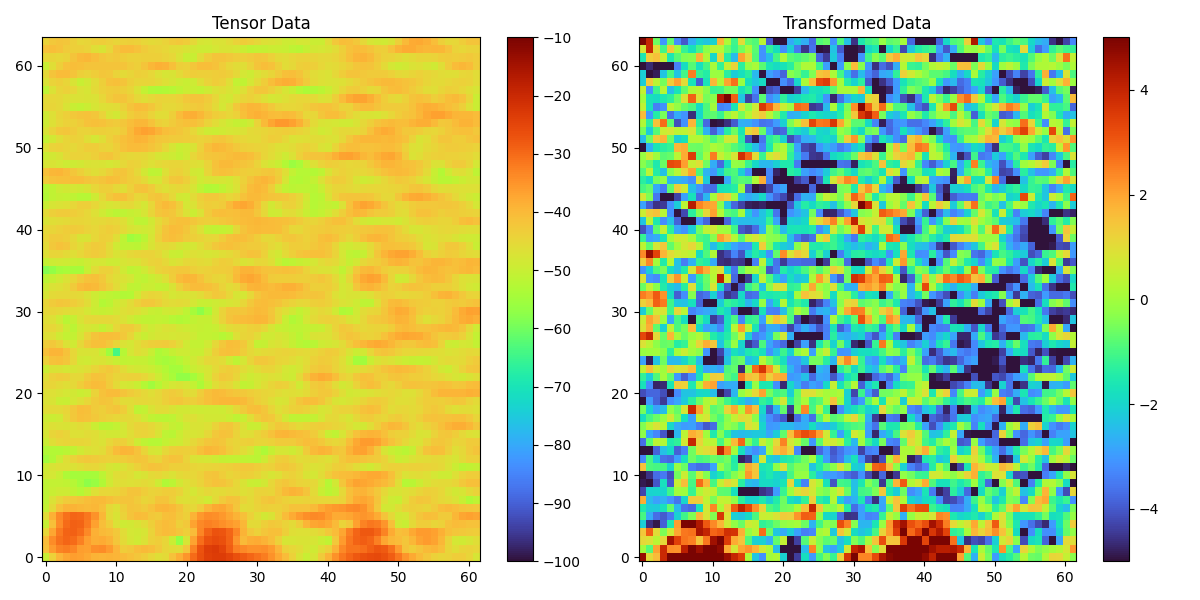
\includegraphics[width=\linewidth]{Bilder/jpg/aug.png}
    \caption{Augmentations of the input tensor}
     \label{aug}
\end{figure}

Figure~\ref{aug} shows the implementation of the augmentation on the input tensor. Augmentations are enhanced for the sake of demonstration. Summarization of each augmentation applied on the data is as follows:
  
These transformations are applied in the custom dataset loader shown in Listing~\ref{lst:binfile_dataset}. PyTorch's recommended pattern is followed for creating a custom dataset from the documentation on PyTorch's website \cite{PyTorch_website}, which allows seamless integration with \texttt{DataLoader} and other utilities. The constructor takes a root directory containing subfolders named after each class (in our case, \texttt{walking} and \texttt{background}), and it builds internal lists of file paths and corresponding integer labels. The \texttt{\_\_len\_\_} method reports the total number of files (i.e.\ the number of samples per epoch), while \texttt{\_\_getitem\_\_} loads each file, applies the STFT-based processing, permutes axes to match PyTorch's \texttt{(C, H, W)} convention, and if a \texttt{transform} is provided it runs the custom augmentations before returning the \texttt{(tensor, label)} pair. This structure cleanly separates I/O, signal preprocessing, and augmentation, making the training loop straightforward.  

\begin{lstlisting}[style=pythonstyle, caption={Custom Dataset for loading and processing footstep files}, label=lst:binfile_dataset]
    class BinFileDataset(Dataset):
        def __init__(self, root_dir: str, event_types: Dict[int, Union[str, List[str]]], transform=None):
            self.root_dir = Path(root_dir)
            self.transform = transform
    
            # labels
            self.event_types = event_types
            self.class_to_idx = {cls_name: idx for idx, cls_name in event_types.items()}
            self.file_list = []
            self.labels = []
    
            self.visualizer = Visualizer()
            for event_idx, event_type in event_types.items():
                subfolders = [event_type] if not isinstance(event_type, list) else event_type
                for subfolder in subfolders:
                    cls_dir = self.root_dir / subfolder
                    if not cls_dir.exists():
                        raise ValueError(f"Subfolder {cls_dir} does not exist.")
                    for file_path in cls_dir.rglob("*"):
                        if file_path.suffix in [".bin", ".npy"]:
                            self.file_list.append(file_path)
                            self.labels.append(event_idx)
            if not self.file_list:
                raise ValueError(f"No data found in {self.root_dir!r}.")
    
        def __len__(self):
            return len(self.file_list)
    
        def __getitem__(self, idx):
            file_path = self.file_list[idx]
            label = int(self.labels[idx])
            if label < 0 or label >= len(self.event_types):
                raise ValueError(f"Invalid label {label} for file {file_path}.")
    
            if file_path.suffix == ".bin":
                with open(file_path, 'rb') as f:
                    data = np.fromfile(f, dtype=np.int64).reshape((length, channels))
            elif file_path.suffix == ".npy":
                data = np.load(file_path)
            else:
                raise ValueError(f"Unsupported file format: {file_path.suffix}")
    
            tensor_data = self.visualizer.data_process(data)
            tensor_data = torch.from_numpy(tensor_data.astype(np.float32)).contiguous()
            tensor_data = tensor_data.permute(1,0,2).contiguous()
    
            if self.transform:
                transformed_data = self.transform(tensor_data)
                return transformed_data, label
            return tensor_data, label
\end{lstlisting}

The \texttt{BinFileDataset} class wraps the extracted data files into an iterable PyTorch dataset, making it easy to load and preprocess samples on the fly.  In Listing~\ref{lst:training_setup}, definition of two event types (\texttt{walking} and \texttt{background}) in the \texttt{event\_types} dictionary is passed to \texttt{BinFileDataset} along with the root data path. Then splitting the resulting dataset into training and validation subsets using an 80/20 split; a \texttt{deepcopy} of the validation set ensures that training time augmentations do not leak into validation.  All custom augmentations (Listing~\ref{lst:custom_augmentations}) plus normalization are applied to the training split, whereas the validation split only undergoes normalization with the precomputed mean and standard deviation.  Each split is wrapped in a \texttt{DataLoader} (with specified \texttt{batch\_size} and \texttt{num\_workers}) to handle batching and parallel I/O.

For the model, we use the \texttt{timm} library to instantiate a backbone network  (\texttt{effici\allowbreak-entnet\_b0.ra\_in1k} or \texttt{convnextv2\_atto.fcmae\_ft\_in1k}) with pretrained weights, specifying the correct number of output classes and input channels. To address class imbalance, we compute per class weights via \texttt{compute\_class\_weight} from scikit learn library  and supply them to a weighted \texttt{CrossEntropyLoss}, which produces per sample losses.  Finally, we optimize the model using the \texttt{Adam} optimizer (adaptive moment estimation) and log training metrics (loss, accuracy, etc.) to TensorBoard via \texttt{SummaryWriter}.

\begin{lstlisting}[style=pythonstyle, caption={Dataset setup and model initialization }, label=lst:training_setup]
    # Define event labels
    event_types = {0: "background", 1: "walking"}
    
    # Create dataset and split
    dataset = BinFileDataset(root_dir='path/to/data', event_types=event_types)
    train_size = int(0.8 * len(dataset))
    val_size   = len(dataset) - train_size
    train_ds, val_ds = random_split(dataset, [train_size, val_size])
    val_ds = deepcopy(val_ds)
    
    # Assign transforms
    train_ds.dataset.transform = transforms.Compose([
        K.Normalize(mean=channel_means, std=channel_stds),
        K.RandomHorizontalFlip(p=1),
        RandomGaussianNoise(mean=0, std=1.5),
        RandomAmplitudeScaling((0.9, 1.1)),
        RandomAffineHorizontalScalePyTorch(scale=0.7, p=1),
    ])
    val_ds.dataset.transform = transforms.Compose([
        K.Normalize(mean=channel_means, std=channel_stds),
    ])
    
    # DataLoaders
    train_loader = DataLoader(train_ds, batch_size=32, num_workers=8, shuffle=True)
    val_loader   = DataLoader(val_ds,   batch_size=32, num_workers=8, shuffle=False)
    
    # Model, loss & optimizer
    model = timm.create_model("efficientnet_b0.ra_in1k", pretrained=True,
                              num_classes=2, in_chans=1).to(device)
    
    weights = compute_class_weight("balanced", classes=np.unique(all_labels), y=all_labels)
    criterion = nn.CrossEntropyLoss(weight=torch.tensor(weights).to(device))
    optimizer = optim.Adam(model.parameters(), lr=1e-4, weight_decay=1e-2)
    \end{lstlisting}

The other important function used before training is \texttt{mixup\_data}, which implements the MixUp augmentation strategy. It samples a mixing coefficient $\lambda \sim \mathrm{Beta}(\alpha,\alpha)$, shuffles each batch, and forms convex combinations of both inputs and labels. Listing~\ref{lst:mixup_data} shows its implementation. During training, the loss is computed as  
\[
\mathcal{L}
= \lambda\,\ell\bigl(f(\widetilde x),y_a\bigr)
+ (1-\lambda)\,\ell\bigl(f(\widetilde x),y_b\bigr),
\]
encouraging smoother decision boundaries and improved generalization.
\begin{lstlisting}[style=pythonstyle, caption={MixUp data augmentation function}, label=lst:mixup_data]

    def mixup_data(x, y, alpha=0.2):
        if alpha > 0:
            lam = np.random.beta(alpha, alpha)
        else:
            lam = 1.0
        batch_size = x.size(0)
        index = torch.randperm(batch_size).to(x.device)
        mixed_x = lam * x + (1 - lam) * x[index]
        y_a, y_b = y, y[index]
        return mixed_x, y_a, y_b, lam
    \end{lstlisting}


The training loop in Listing~\ref{lst:train_loop} runs for a fixed number of epochs. At the start of each epoch, the model is set to training mode and the running loss and accuracy meter are reset. For each mini-batch, inputs and labels are moved to the GPU, mixed via MixUp (producing \texttt{targets\_a}, \texttt{targets\_b}, and \texttt{lam}), and passed through the network. The combined MixUp loss is computed, backpropagated, and the Adam optimizer updates the weights. Accumulation of batch losses and updating the training accuracy meter is done, then computation and logging the average training loss and accuracy to TensorBoard.

After training, model is switched to evaluation and gradients are disabled. Looping over the validation loader, computing over the standard cross-entropy loss per batch, updating the validation accuracy meter, and accumulating losses is done. At epoch end, the average validation loss and accuracy are computed and logged. Once all epochs complete, a checkpoint containing the model's state dict, the optimizer's state dict, and the class-to-index mapping is saved for future use.  
    

    \begin{lstlisting}[style=pythonstyle, caption={Core training and validation loop}, label=lst:train_loop]
    def train(num_epochs=65):
        train_acc = Accuracy(num_classes=2).to(device)
        val_acc   = Accuracy(num_classes=2).to(device)
        # Initialize optimizer, criterion, writer
        
            for epoch in range(num_epochs):
                model.train()
                running_loss = 0.0
                train_acc.reset()
        
                for inputs, labels in train_loader:
                    inputs, labels = inputs.to(device), labels.to(device)
                    inputs, targets_a, targets_b, lam = mixup_data(inputs, labels, alpha=0.2)
        
                    optimizer.zero_grad()
                    outputs = model(inputs)
                    loss = lam*criterion(outputs, targets_a) \
                         + (1-lam)*criterion(outputs, targets_b)
                    loss.backward()
                    optimizer.step()
        
                    running_loss += loss.item()
                    train_acc.update(outputs, labels)
        
                epoch_train_loss = running_loss / len(train_loader)
                train_accuracy  = train_acc.compute().item()
                writer.add_scalar('Train/Loss',     epoch_train_loss, epoch)
                writer.add_scalar('Train/Accuracy', train_accuracy,   epoch)
        
                model.eval()
                val_loss = 0.0
                val_acc.reset()
        
                with torch.no_grad():
                    for inputs, labels in val_loader:
                        inputs, labels = inputs.to(device), labels.to(device)
                        outputs = model(inputs)
                        val_loss += criterion(outputs, labels).item()
                        val_acc.update(outputs, labels)
        
                epoch_val_loss = val_loss / len(val_loader.dataset)
                val_accuracy   = val_acc.compute().item()
                writer.add_scalar('Val/Loss',     epoch_val_loss, epoch)
                writer.add_scalar('Val/Accuracy', val_accuracy,   epoch)
        
            torch.save({
                'model': model.state_dict(),
                'optimizer': optimizer.state_dict(),
                'class_to_idx': dataset.class_to_idx
            }, 'checkpoint.pth')
        \end{lstlisting}

Using the structure explained in the above listings the ConvNext V2 and EfficientNet models are trained using the 1 spatial channel and 10 spatial channel data. The logs which save Loss and Accuracy are monitored to see if the model are trained properly.  

\subsection{Testing of the model}
The trained models have the checkpoints saved. The checkpoints have the weights saved for the model. The model is tested using the evaluation mode to see how the model performs. Listing~\ref{lst:test_loop} shows the core evaluation script used to assess model performance on held-out data.

\begin{lstlisting}[style=pythonstyle, caption={Model test script}, label=lst:test_loop]
    # Set random seed and load checkpoint
    torch.manual_seed(42)
    checkpoint = torch.load('effnet_with_preprocess_1d_v1.pth', weights_only=True)
    
    # Prepare test dataset and loader
    event_types = {0: "background", 1: "walking"}
    transform = transforms.Compose([K.Normalize(mean=checkpoint['mean'], std=checkpoint['std'])])
    test_ds = BinFileDataset(root_dir='path/to/test', event_types=event_types, transform=transform)
    test_loader = DataLoader(test_ds, batch_size=32, num_workers=8, shuffle=False)
    
    # Model setup
    model = timm.create_model("efficientnet_b0.ra_in1k", pretrained=True,
                              num_classes=2, in_chans=1)
    model.load_state_dict(checkpoint['model_state_dict'])
    device = torch.device('cuda' if torch.cuda.is_available() else 'cpu')
    model.to(device).eval()
    
    # Metrics and loss
    criterion    = nn.CrossEntropyLoss(reduction='none')
    test_acc     = Accuracy(task="multiclass", num_classes=2).to(device)
    test_confmat = ConfusionMatrix(task="multiclass", num_classes=2).to(device)
    
    # test loop
    test_loss = 0.0
    samples   = 0
    with torch.no_grad():
        test_acc.reset()
        test_confmat.reset()
        for inputs, labels in test_loader:
            inputs, labels = inputs.to(device), labels.to(device)
            inputs = inputs.permute(0,2,3,1,4).squeeze(3)
            outputs = model(inputs)
            test_loss += criterion(outputs, labels).sum().item()
            samples   += labels.size(0)
            preds = predict_with_threshold(outputs, 0.6)
            test_acc.update(preds, labels)
            test_confmat.update(preds, labels)
    
    # Final metrics
    avg_loss = test_loss / samples
    acc      = test_acc.compute().item()
    conf_mat = test_confmat.compute().cpu().numpy()
    
    print(f"Test Loss: {avg_loss:.4f}, Accuracy: {acc*100:.2f}%")
    print(f"Confusion Matrix:\n{conf_mat}")
    \end{lstlisting}
    
In first step the random seed of reproducibility which is used for setting the random numbers. Setting the seed ensures that all subsequent calls to PyTorch's random number generator produce the same sequences, making the evaluation fully reproducible. The saved checkpoint is loaded, which contains the model weights as well as the normalization statistics (mean and standard deviation). The test dataset is constructed using the \texttt{BinFileDataset} from the listing~\ref{lst:binfile_dataset} where the location for the test set and normalizing using the parameters from the checkpoint. A \texttt{DataLoader} wraps this dataset with a batch size of 32 and multiple worker processes for parallel I/O. 

Next, the model is setup to (\texttt{efficientnet\_b0.ra\_in1k} or \texttt{convnextv2\allowbreak\_atto.fcmae\_ft\_in1k}) using the \texttt{timm.create\_model} and setting the channels and classes are set with the same numbers. The model is moved to evaluation mode and the loss function is initializated using \texttt{CrossEntropyLoss} and key metrics like accuracy and confusion matrix are taken from \texttt{torchmetrics}~ \cite{torchmetrics} necessary to evaluate the performance of the model.

The evaluation loop (with gradients disabled) mirrors the validation phase from Listing~\ref{lst:train_loop}.  We iterate over the test loader, compute the standard cross-entropy loss for each batch, and update metrics such as accuracy and the confusion matrix to assess model performance.  Finally, we apply the \texttt{predict\_with\_threshold} function which returns "walking" only if the activity probability exceeds a chosen cutoff and otherwise returns "background" to convert soft outputs into discrete class labels.

\subsection{Comparison of training, validation and testing performance}
\label{sec:comp}
The models are trained and tested with scripts and datasets as seen in the previous sections. The tensorboard logging is used to log the graphs of loss and accuracy. The four different types of checkpoints, which are trained and evaluated on the respective dataset. Ideally the loss should be around 0 and accuracy should be near 100\%.

The graphs~\ref{conv_1d_train} show the loss and accuracy plots for training and validation on dataset-1D of ConvNext V2 model. The training is done over 65 epochs. Training loss (blue) starts at 0.37 which falls rapidly after first 10 epochs and oscillates between 0.18 and 0.25. Validation loss (orange) starts at 0.21 and steadily declines to around 0.12 indicating model continues to improve on unseen data even after traing loss plateaus. Training accuracy (blue) climbs from around 68\% to 80\% but shows some fluctuations once loss stabilizes. Validation accuracy (orange) starts at around 92\% and rises to 95\% remaining consistently high demonstarting good generalization.

\begin{figure}[h]
    \centering
    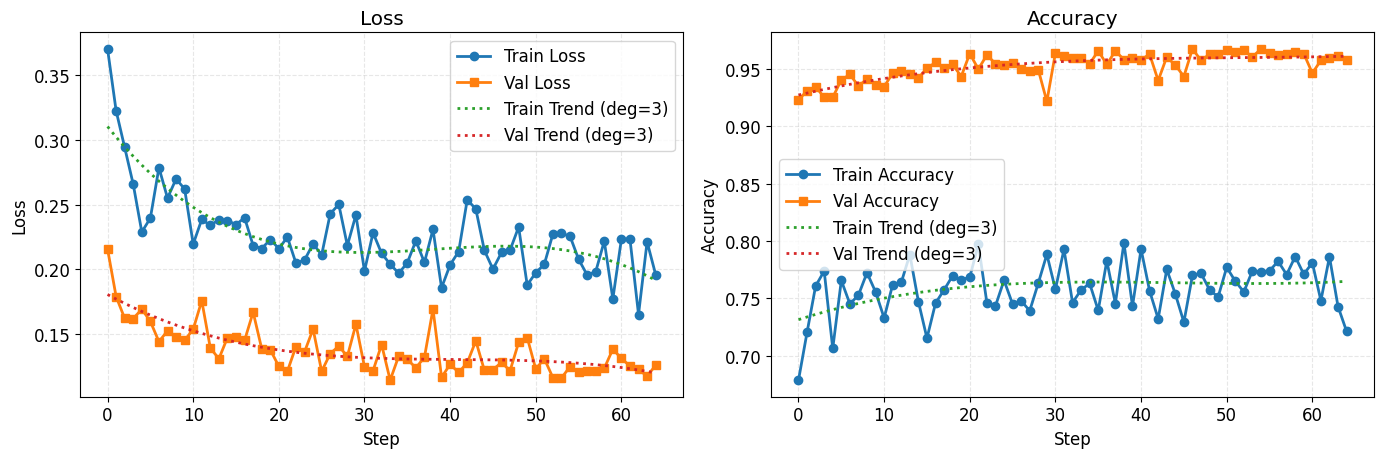
\includegraphics[width=\linewidth]{Bilder/jpg/conv_1d_train.png}
    \caption{Loss and Accuracy plots for training and validation for ConvNext V2 on dataset-1D}
    \label{conv_1d_train}
\end{figure}

Table~\ref{conv_1d_test} summarizes the ConvNext model's performance on the dataset-1D. The overall test loss of 0.36 and accuracy of 87.55\% indicate that the model generalizes well to held-out examples. From the confusion matrix (lower block of the table), we see that of 1591 true background samples the model correctly labels 1454 (91.4\% recall) and of 987 true walking events it correctly labels 803 (81.4\% recall). Precision scores 88.8\% for background and 85.4\% for walking confirming the model makes relatively few false alarms in each class.

\begin{table}[ht]
    \centering
    \caption{Test results for the ConvNext V2 model on the dataset-1D}
    \label{conv_1d_test}
    \begin{tabular}{lcc}
      \toprule
      \textbf{Metric}            & \textbf{Background} & \textbf{Walking} \\
      \midrule
      Test Loss                  & \multicolumn{2}{c}{0.3625}          \\
      Test Accuracy (\%)         & \multicolumn{2}{c}{87.55}           \\
      \addlinespace
      \multicolumn{3}{l}{\textbf{Confusion Matrix}} \\
      \quad True Background      & 1454                & 137             \\
      \quad True Walking         & 184                 & 803             \\
      \addlinespace
      \multicolumn{3}{l}{\textbf{Per-class Precision, Recall, F1 (\%)}} \\
      Precision                  & 88.77               & 85.43           \\
      Recall                     & 91.39               & 81.36           \\
      F1 Score                   & 90.06               & 83.34           \\
      \bottomrule
    \end{tabular}
  \end{table}
  
The graphs~\ref{eff_1d_train} show the loss and accuracy plots for training and validation of EfficientNet model on dataset-1D. Over 65 epochs, training is done. The train loss (blue) starts at 3.05 and gradually drops till it reaches 0.281. The validation loss (orange) starts at around 2 and gradually drops till it reaches 0.18. The minor spike is observed around 30th epoch but recover quickly. The train accuracy (blue) rises from 64\% to 75\% reflecting incremental learning. The validation accuracy (orange) starts at 72\% and rises till 90\% while plateauing between 88\% and 93\%. The learning summarizes good generalization.

\begin{figure}[h]
    \centering
    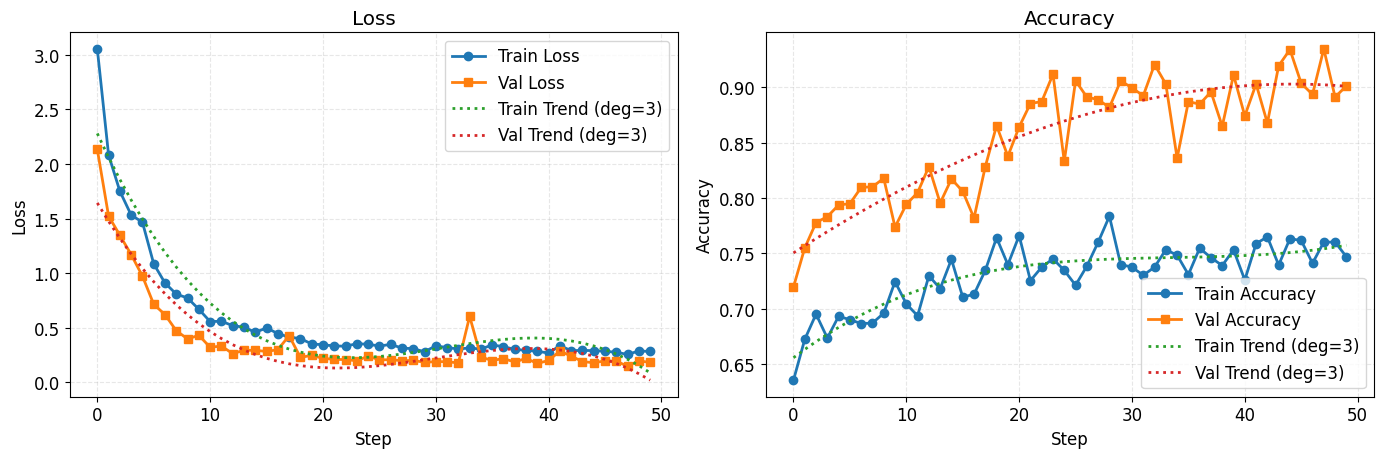
\includegraphics[width=\linewidth]{Bilder/jpg/eff_1d_train.png}
    \caption{Loss and Accuracy plots for training and validation for EfficientNet on dataset-1D}
    \label{eff_1d_train}
\end{figure}

\begin{table}[ht]
    \centering
    \caption{Test results for the EfficientNet model on dataset-1D}
    \label{eff_1d_test}
    \begin{tabular}{lcc}
      \toprule
      \textbf{Metric}            & \textbf{Background} & \textbf{Walking} \\
      \midrule
      Test Loss                  & \multicolumn{2}{c}{0.2496}          \\
      Test Accuracy (\%)         & \multicolumn{2}{c}{91.89}           \\
      \addlinespace
      \multicolumn{3}{l}{\textbf{Confusion Matrix}} \\
      \quad True Background      & 1512                & 79              \\
      \quad True Walking         & 130                 & 857             \\
      \addlinespace
      \multicolumn{3}{l}{\textbf{Per-class Precision, Recall, F1 (\%)}} \\
      Precision                  & 92.08               & 91.56           \\
      Recall                     & 95.03               & 86.83           \\
      F1 Score                   & 93.54               & 89.13           \\
      \bottomrule
    \end{tabular}
  \end{table}
  
Table \ref{eff_1d_test} reports the EfficientNet models performance on the dataset-1D. The model achieves a test loss of 0.25 and overall accuracy of 91.89\%, demonstrating strong generalization. Examining the confusion matrix, 95.0\% of true background samples (1512 out of 1591) are correctly identified, while 86.8\% of true walking events (857 out of 987) are detected. Precision remains high for both classes 92.1\% for background and 91.6\% for walking indicating few false alarms. Finally, F1 scores of 93.5\% and 89.1\% reflect a solid balance between precision and recall in each category.

The graph~\ref{conv_2d_train} shows the training and validation loss and accuracy plots of ConvNext V2 model on dataset-2D. The train loss (blue) and validation loss (orange) declines steeply where train loss drops from 0.56 to 0.20 at epoch 3 and validation loss plunges even faster from 0.88 to 0.06 at epoch 2. Train loss sees occasianl small upticks at epoch 5 but stablizes later. Validation loss remians low with tiny spikes at around epochs 11 and 21. Train accuracy (blue) starts around 57\% and reaches 85\% at epoch 10 then osscilates between 82\%-87\%. Validation accuracy (orange) skyrockets to 99\% at epoch 3 and stay high with some minor dips at around at epoch 11 and 21 suggesting good learning. 

\begin{figure}[h]
    \centering
    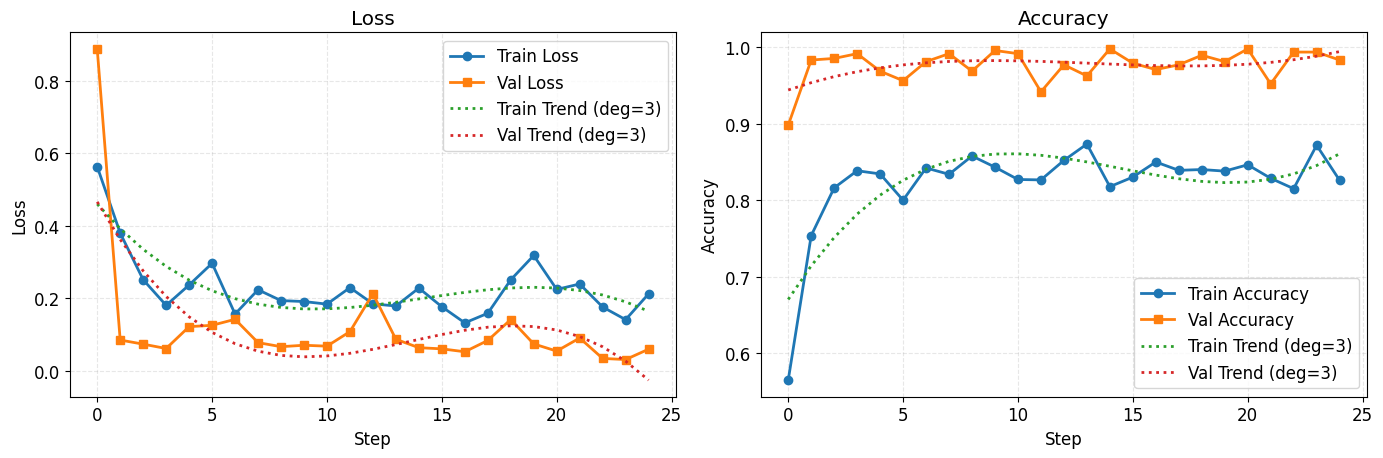
\includegraphics[width=\linewidth]{Bilder/jpg/conv_2d_train.png}
    \caption{Loss and Accuracy plots for training and validation for ConvNext V2 with 10 spatial channels and 2 sample length}
    \label{conv_2d_train}
\end{figure}

\begin{table}[ht]
    \centering
    \caption{Test results for the ConvNeXt V2 model on the dataset-2D}
    \label{conv_2d_test}
    \begin{tabular}{lcc}
      \toprule
      \textbf{Metric}            & \textbf{Background} & \textbf{Walking} \\
      \midrule
      Test Loss                  & \multicolumn{2}{c}{0.0537}          \\
      Test Accuracy (\%)         & \multicolumn{2}{c}{99.48}           \\
      \addlinespace
      \multicolumn{3}{l}{\textbf{Confusion Matrix}} \\
      \quad True Background      & 1678                & 4               \\
      \quad True Walking         & 5                   & 58              \\
      \addlinespace
      \multicolumn{3}{l}{\textbf{Per-class Precision, Recall, F1 (\%)}} \\
      Precision                  & 99.70               & 93.55           \\
      Recall                     & 99.76               & 92.06           \\
      F1 Score                   & 99.73               & 92.80           \\
      \bottomrule
    \end{tabular}
  \end{table}

Table~\ref{eff_2d_test} presents the ConvNext V2 model's performance on the dataset-2D. The extremely low test loss of 0.0537 and very high overall accuracy of 99.48\% show that the model almost perfectly separates footsteps from background. In the confusion matrix, 1678 out of 1682 background samples are correctly classified (99.8\% recall), and 58 out of 63 walking events are detected (92.1\% recall). Precision remains excellent 99.7\% for background and 93.6\% for walking indicating virtually no false alarms in the background class and very few in the walking class. The resulting F1 scores (99.7\% for background, 92.8\% for walking) confirm a close to ideal balance of precision and recall.

The graph~\ref{eff_2d_train} shows the train loss and accuracy set for ConvNeXt V2 on dataset-2D. The model runs over 25  epochs. The train loss (blue) and validation loss (orange) have a rapid intial drops over first 3-4 epochs indicating model picks up on low-level features. After that decline is more gradual and settles at 0.2 to 0.3. The sharp spike at epochs 11-12 suggesting model destabilzes then model recovers. Train accuracy (blue) rises from 63\% to 80\% and pleateauing at the point. Validation accuracy (orange) jumps from 66\% to 91\% which dips at epoch 4 to 58\% then agian recovers. The graph demonstarates the good genralization over the data.

\begin{figure}[h]
    \centering
    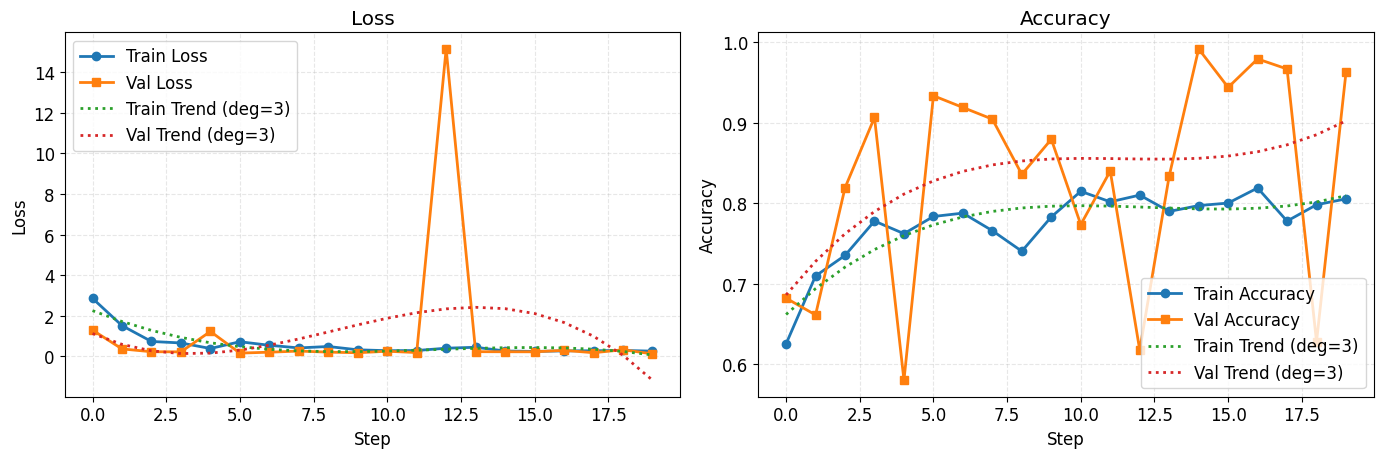
\includegraphics[width=\linewidth]{Bilder/jpg/eff_2d_train.png}
    \caption{Loss and Accuracy plots for training and validation for EfficientNet with 10 spatial channels and 2 sample length}
    \label{eff_2d_train}
\end{figure}

\begin{table}[ht]
    \centering
    \caption{Test results for the EfficientNet model on the 2-D dataset}
    \label{eff_2d_test}
    \begin{tabular}{lcc}
      \toprule
      \textbf{Metric}            & \textbf{Background} & \textbf{Walking} \\
      \midrule
      Test Loss                  & \multicolumn{2}{c}{0.0934}          \\
      Test Accuracy (\%)         & \multicolumn{2}{c}{99.48}           \\
      \addlinespace
      \multicolumn{3}{l}{\textbf{Confusion Matrix}} \\
      \quad True Background      & 1679                & 3               \\
      \quad True Walking         & 6                   & 57              \\
      \addlinespace
      \multicolumn{3}{l}{\textbf{Per-class Precision, Recall, F1 (\%)}} \\
      Precision                  & 99.64               & 95.00           \\
      Recall                     & 99.82               & 90.48           \\
      F1 Score                   & 99.73               & 92.68           \\
      \bottomrule
    \end{tabular}
  \end{table}

Table~\ref{eff_2d_test} summarizes the EfficientNet model's performance on dataset-2D With a test loss of only 0.934 and an overall accuracy of 99.48\%, the network distinguishes footsteps from background almost flawlessly. The confusion matrix shows that 1679 out of 1682 background samples are correctly identified (99.8\% recall), while 57 out of 63 walking events are detected (90.5\% recall). High precision values 99.6\% for background and 95.0\% for walking indicate very few false positives. Finally, F1 scores of 99.7\% and 92.7\% confirm an excellent balance between precision and recall for each class.

The metrics in the graphs suggests that models shows the similar performance over the testing set for the same models training set. Except the ConvNext V2 model on dataset-1D, all the other show similar performance and are better than ConvNext V2 model on dataset-1D. The checkpoints should be evaluated on real-time across the data stream coming in through the DAS configurator application. Model should show similar performance as the performance on testing set. 

\section{Real-time evaluation Framework}
\label{sec:realtime_evaluation}
For real time evaluation of the model, the data needs to be streamed to the model and based on the data the model is able to classify the data. This is done with the help of \texttt{spectrogram\_classifier} module which is used for the real-time evaluation and developed with the help of \texttt{dasdpu} package. The \texttt{dasdpu} package is an internal package developed at AP Sensing for running and testing algorithms on DAS DPU or locally on HDF5 files. It is used for socket reading of Frequency Band Energy (FBE) and/or phases data. It also sends the events or alarms to the DPU such that are displayed in the Configurator. This package is one of the most important elements in the real-time evaluation script.

Spectrogram Classifier (\texttt{spectrogram\_classifier}) is the module developed internally at AP Sensing which is used for evaluation of the models. The module implements the online execution of the logic for the phase-based footstep detection. It ingests the raw phase samples from the DAS-acquisition service, buffers a short user-defined time window, and optionally computes the spectrograms for each channel before forwarding them to the trained model. When the model's output probability exceeds the user-set threshold, the pipeline emits a detection. The detections are tracked over time by grouping and assigning them track IDs, thus allowing the tracking of a moving disturbance along the cable. Once a track accumulates sufficient repeated detections (confidence), the alarm is raised. Figure~\ref{dg_spectrogram} gives an overview of the structure of the \texttt{spectrogram\_classifier} module and it's dependencies to all other packages. All the standard python libraries on which the module is dependant on are excluded. The dependencies with \texttt{dasdpu} and other packages is shown in the figure~\ref{dg_spectrogram}. The \texttt{system.py} is the file which which has all the logic files essential for the working of the module and is the file where all the changed files are imported. 

\begin{figure}[h]
    \centering
    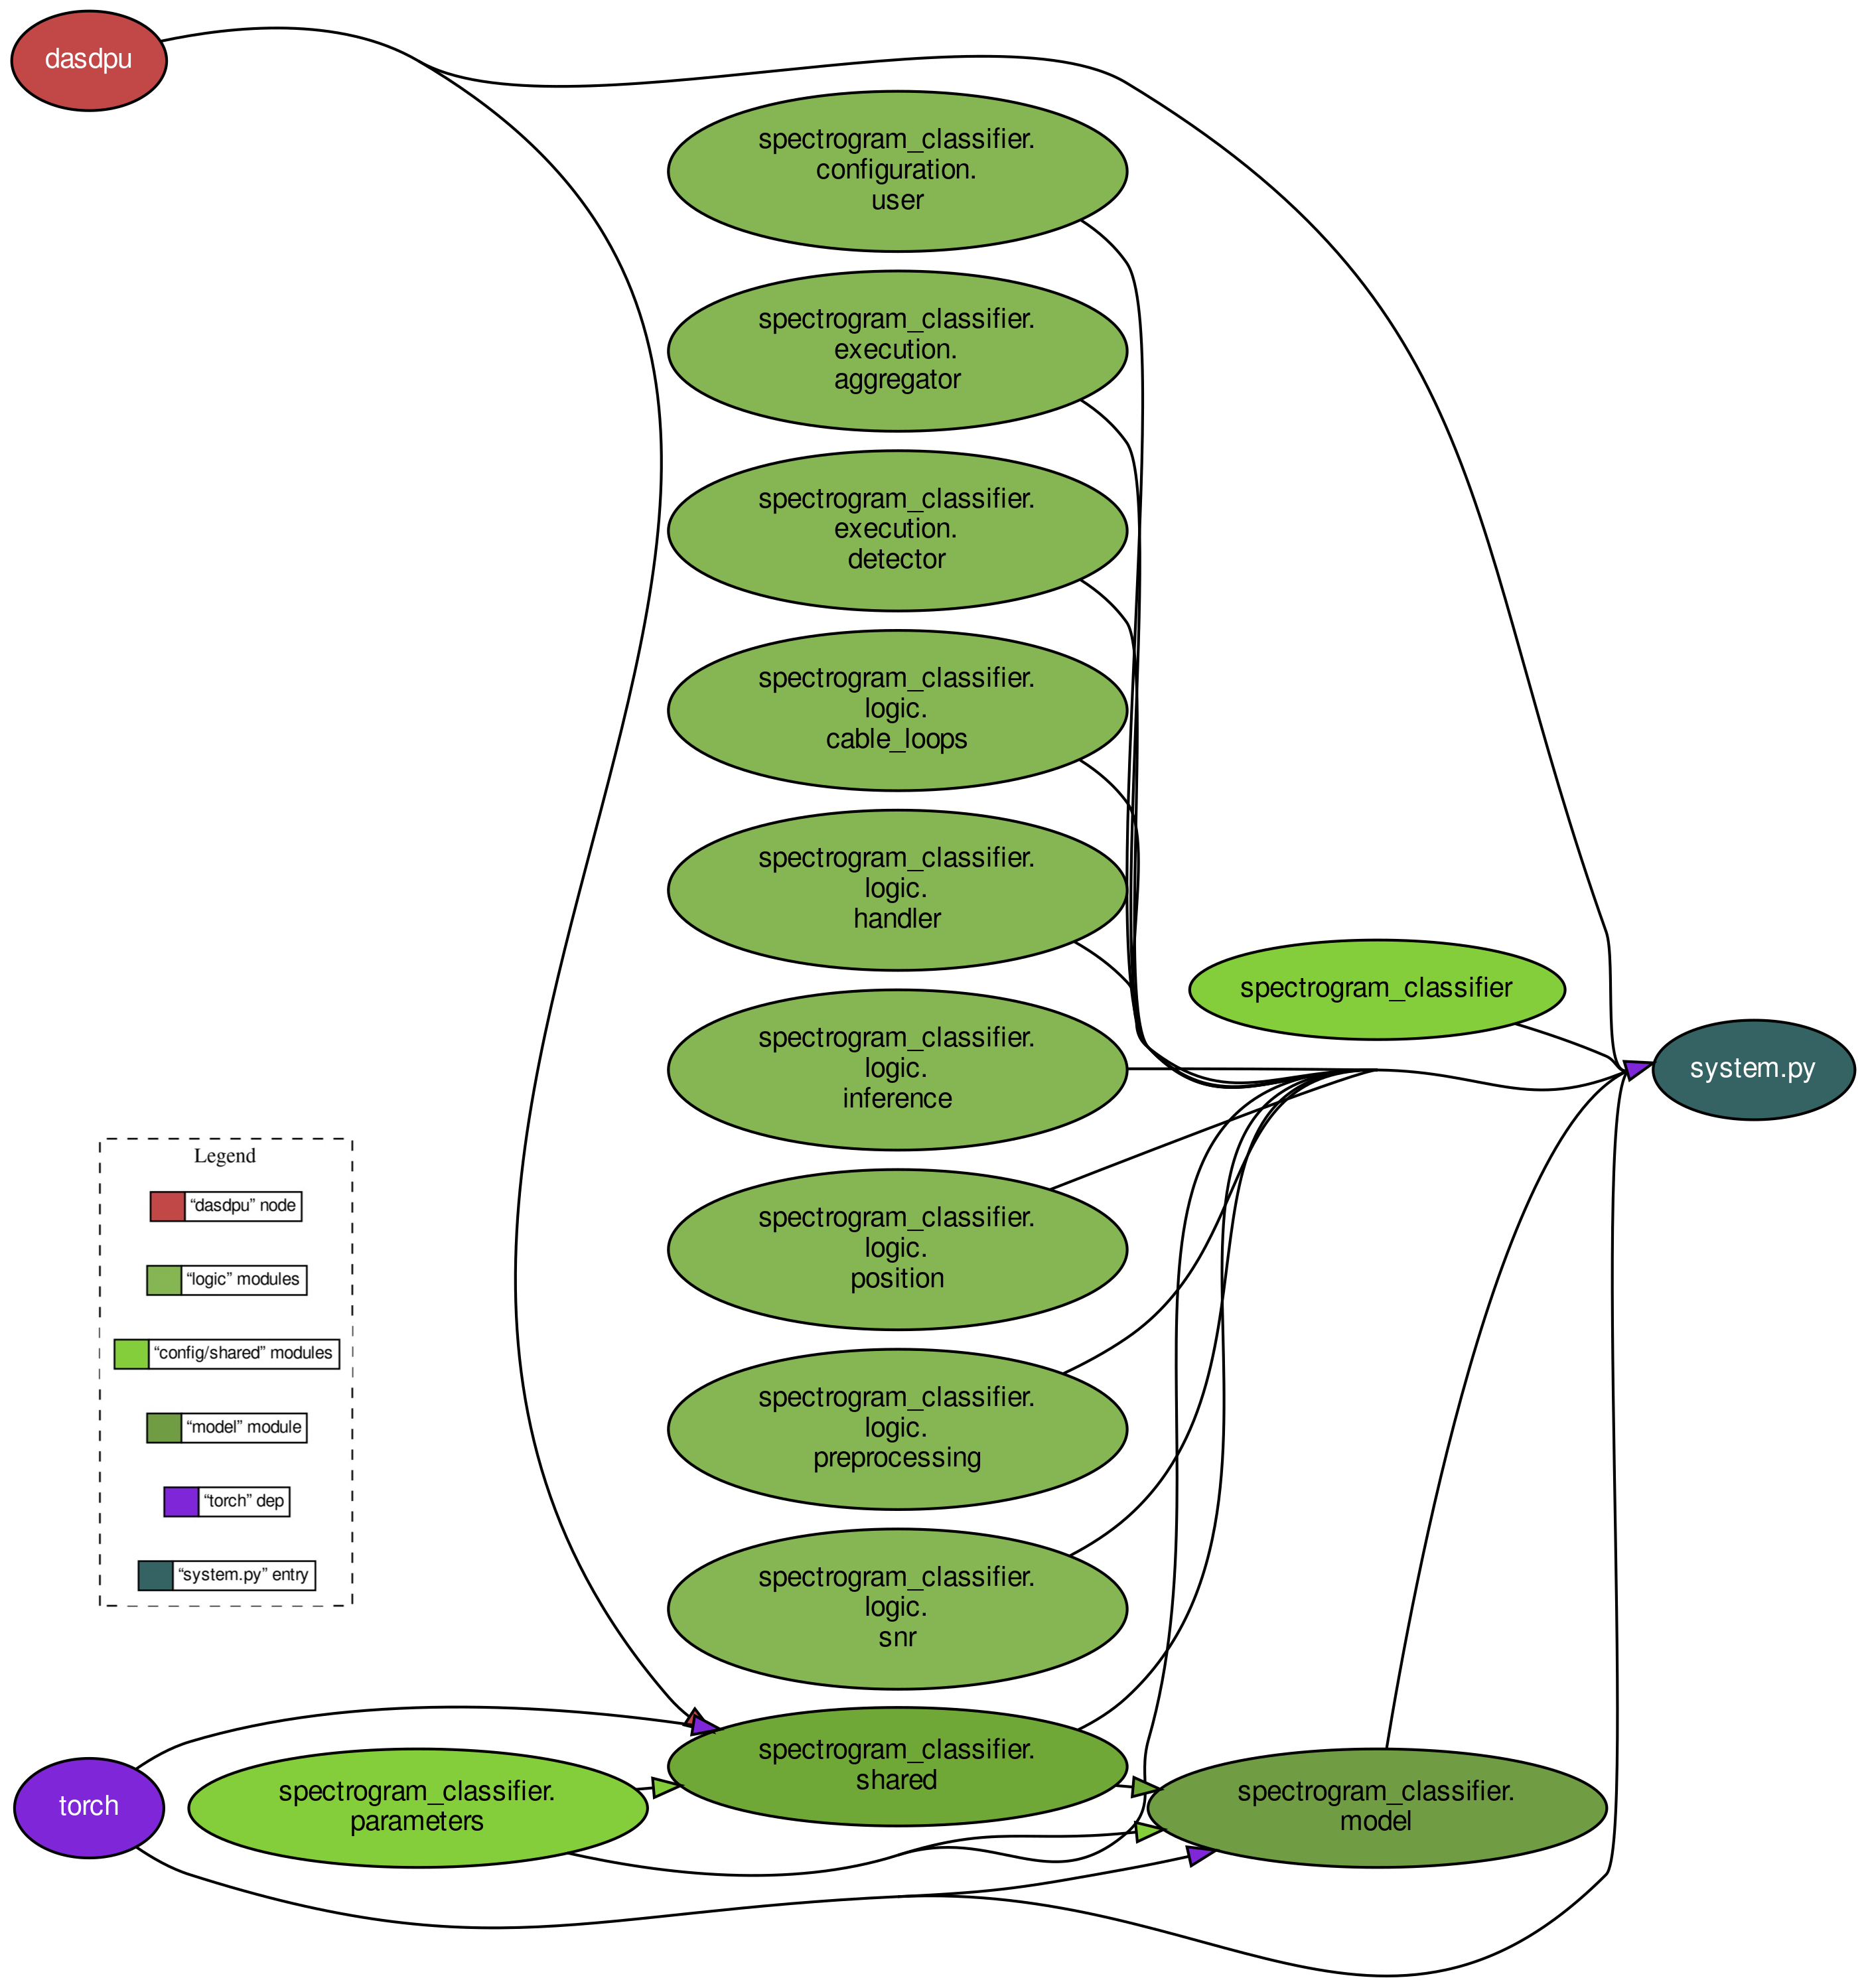
\includegraphics[width=\linewidth]{Bilder/jpg/output_graph.png}
    \caption{Dependency Graph of \texttt{spectrogram\_classifier} module}
    \label{dg_spectrogram}
\end{figure}

The \texttt{spectrogram\_classifier.execution.aggregator} and \texttt{spectrogram\_classifier.execution.detector} are the top level files responsible for the execution. The \texttt{spectrogram\_classifier.logic.inference} returns the list of detections from the tensor. Position in terms of distance is mapped from \texttt{spectrogram\_classifier.logic.position} from the spatial channels. All the remaining files are not crucial for detection but serve as the support and enables in smooth running of the system. The \texttt{spectrogram\_classifier} module is edited to adjust for the preprocessing steps done while training the model and models ConvNext V2 and EfficientNet are also added in the pipeline for easy selection and switching. The preprocessing section is inserted in the \texttt{spectrogram\_classifier.logic.preprocessing} which is same as the training. The model is inserted in the \texttt{spectrogram\_classifier.model} is also same as the training.

\begin{lstlisting}[style=pythonstyle, caption={Preprocessing for conversion of raw phase data to spectrogram in the framework}, label=lst:stft_processing]
class SpectrogramPreprocessorStft:
    def __init__(self, model_params: Parameters, data_rate_hz: int = 1000, device: torch.device = torch.device("cuda")):
        self._data_rate_hz = data_rate_hz
        self._device = device
        self._multiplier = data_rate_hz // 500
        self._nperseg = 128 * self._multiplier
        self._noverlap = self._nperseg - 14 * self._multiplier
        self._f_bank = (
            melscale_fbanks(
                n_freqs=self._nperseg // 2 + 1,
                f_min=model_params.f_min,
                f_max=model_params.f_max,
                n_mels=model_params.n_mels,
                sample_rate=data_rate_hz,
                mel_scale="htk",
                norm=None,
            )
            .cpu()
            .numpy()
        )

    def preprocess(self, data: np.ndarray, axis: int) -> tuple[np.ndarray, np.ndarray]:
        data_accum = self._accum(data, axis=axis)
        f, t, stft = signal.stft(
            data_accum,
            fs=self._data_rate_hz,
            nperseg=self._nperseg,
            noverlap=self._noverlap,
            padded=False,
            scaling="psd",
            axis=axis,
        )
        stft = np.abs(stft) ** 2
        stft = np.matmul(stft.transpose((0, 2, 1)), self._f_bank).transpose((0, 2, 1))
        mag = 10 * np.log10(stft)
        return 

    def process(self, tensor_data: torch.Tensor) -> torch.Tensor:  
        tensor_numpy = tensor_data.cpu().numpy()
        numpy_result = self.data_process(tensor_numpy, axis=-1)
        return torch.from_numpy(numpy_result).float().cuda()  

    def _accum(self, x: np.ndarray, axis: int) -> np.ndarray:
        x = np.cumsum(x, axis=axis, dtype=np.int64).astype(np.float32) * INT_TO_RADIANS
        sos = signal.butter(2, 5, "hp", fs=1000, output="sos")
        x = signal.sosfiltfilt(sos, x, axis=axis)
        return x

    @property
    def device(self) -> torch.device:
        return self._device

\end{lstlisting}

The listing~\ref{lst:stft_processing} shows the processing which is same as the listing in the section listing~\ref{lst:mag_processing}. The main difference is that data is in the form a tensor in listing~\ref{lst:stft_processing} so it first needs to be converted into a numpy for the STFT function which is used in preprocessing in training pipeline. After the STFT function in \texttt{preprocess} the shape needs to be considered as the streamed data for realtime since it needs to be in the format \texttt{[batch, frequency\_bins, time]} in comparison to training where the shape is adjusted after extracting the data in listing~\ref{lst:binfile_dataset}. The \texttt{\_accum} function has the cumulative sum where it is done on the time axis as the data distorts and the model will not be able to do the detections.

\begin{lstlisting}[style=pythonstyle, caption={Model evaluation mode in the framework}, label=lst:model_rt]
def get_effnet_b0(params: Parameters) -> torch.nn.Module:
    return timm.create_model("efficientnet_b0", num_classes=params.n_classes, in_chans=params.model_n_channels)

def get_convnextv2(params: Parameters) -> torch.nn.Module:
    return timm.create_model("convnextv2_atto", num_classes=params.n_classes, in_chans=params.model_n_channels)

def create(cls, weights_path: str | Path, device=torch.device("cpu")) -> Model:

    model_data = torch.load(weights_path)
    state_dict = model_data["model_state_dict"]
    mean = model_data["mean"]
    std = model_data["std"]

    params = Parameters(
        epochs=100,
        batch_size=32,
        test_batch_size=32,
        learning_rate=1e-3,
        weight_decay=1e-4,
        dataset_mean=mean.reshape((1, 1, 1, 1)),
        dataset_std=std.reshape((1, 1, 1, 1)),
        label_smoothing=0.1,
        accum_phase=False,
        highpass_cutoff_hz=None,
        expected_data_rate_hz=1000,
        n_fft=512,
        hop_size=256,
        pad=0,
        center=True,
        mel_scale=False,
        n_mels=64,
        f_min=0,
        f_max=500,
        model_name="effnet-b0",
        model_d=64,
        n_classes=2,
        model_n_channels=10,
        normalization="global",
    )

    model = create_model(params, state_dict)
    model = TimmModelWrapper(model, mean=mean, std=std)
    model = model.eval()

    return cls(model, device, params)

\end{lstlisting}

The listing~\ref{lst:model_rt} shows the evaluation mode for ConvNext V2 and EfficientNet. These functions are used in the top layer of the model where the parameters like classes and input channels are given to the functions from parameters that are used. The  parameters used in the model are set to the same values which are used while training. The mean and standard deviation calculated during the training ans stored in the checkpoint are extracted and used for normalization of data. The model is created using \texttt{create\_model} function which calls either \texttt{get\_convnextv2} or \texttt{get\_effnet\_b0} based on the model name. The model is wrapped in \texttt{TimmModelWrapper} which is used to adjust the shape and set the normalization parameters. The model is then set to evaluation mode for returning detections
